% $Author$ $Date$

%%%% for public version, toggle \draftfalse in setup2modes.tex
%    (that removes all comments, the blog)

% siminos/cgang/2modes.tex    this is master file:    pdflatex 2modes
%     then:    pdflatex def2modes; bibtex def2modes; pdflatex def2modes; pdflatex def2modes

\documentclass[aip,cha,
%reprint,
secnumarabic,
nofootinbib, tightenlines,
nobibnotes, showkeys, showpacs,
groupedaddress,
preprint,%
%author-year,%
%author-numerical,%
]{revtex4-1}

\newcommand{\version}{atlas ver. 0.3, Aug  1 2012}
% Predrag                   ver. 0.2, Apr 30 2012}
% Predrag from atlas12      ver. 1.1, Apr 25 2012}

        \input setup2modes
        \input ../inputs/def
        \input def2modes

\begin{document}

\title[Low-dimensional cartography]
{Cartography of a 4-dimensional flow: A visual guide to sections and slices}

\author{Daniel Borrero-Echeverry}
\email{borrero@gatech.edu.}
\author{Keith M. Carroll}
\author{Predrag Cvitanovi\'{c}}
% \author{Bryce Robbins} %no response by 2012-07-26, removed
\author{Evangelos Siminos}
% \author{Lei Zhang} %no response by 2012-07-26, removed
\affiliation{
 School of Physics and Center for Nonlinear Dynamics,
 Georgia Inst. of Technology,
 Atlanta, GA  30332, USA
}
    \ifdraft
\date{\today}
    \else
\date{1 May 2012}
%\affiliation{
% School of Physics and School of Mathematics,
% Georgia Inst. of Technology,
% Atlanta, GA  30332, USA
% \\\\
% Georgia Tech PHYS 7224 spring 2012 course project
% \\
% \emph{Advisers:
% Predrag Cvitanovi\'{c},
% Daniel Borrero-Echeverry
% and
% Evangelos Siminos}
%}
   \fi


    \begin{abstract}
Symmetry reduction by the method of slices [blah blah]
the role they play in organizing chaos.
    \end{abstract}

\pacs{02.20.-a, 05.45.-a, 05.45.Jn, 47.27.ed, 47.52.+j, 83.60.Wc}
\keywords{
symmetry reduction,
equivariant dynamics,
relative equilibria,
relative periodic orbits,
slices,
moving frames
}
\maketitle

%\ifdraft\onecolumngrid % 2012-08-06 temporary \onecolumngrid


    \begin{quotation}
Today, it is possible to  [blah blah].
    \end{quotation}

\section{Introduction}
\label{s:intro}

Over the last decade, new insights into the dynamics of  [blah blah]

Our goals here are two-fold:
(i)  [blah blah].
(ii) [blah blah].

As a motivation, consider the chaotic dynamics exhibited by the
small-cell \KS\ system studied in \refref{lanCvit07}. Examination of
typical long-time simulations shows that the spatio-temporal chaos arises
from visits to two kinds of unstable patterns, a `central wobble' region
$S_C$, and a symmetric pair of right/left `drifts' $\{S_L,S_R\}$. In
\statesp\ projections orbits stay in one neighborhood for a while, then
hop to another neighborhood, as illustrated in \reffig{f:antlong}. The
strange attractor that they explore is curved and folded in such a way
that a single local linear chart cannot cover the whole attractor,
several charts are needed, as illustrated by \reffig{fig:2ModeAtlas}\,(d).

The \statesp s of \KS\ and fluid-dynamical flows are high\dmn\ and
difficult to visualize, so here we shall illustrate the key ideas by a
much simpler example, the $\SOn{2}$-equivariant  \twoMode\ system.

%%%%%%%%%%%%%%%%%%%%%%%%%%%%%%%%%%%%%%%%%%%%%%%%%%%%%%%%%%%%
\begin{figure} %[tbp] %[h]
    \centering
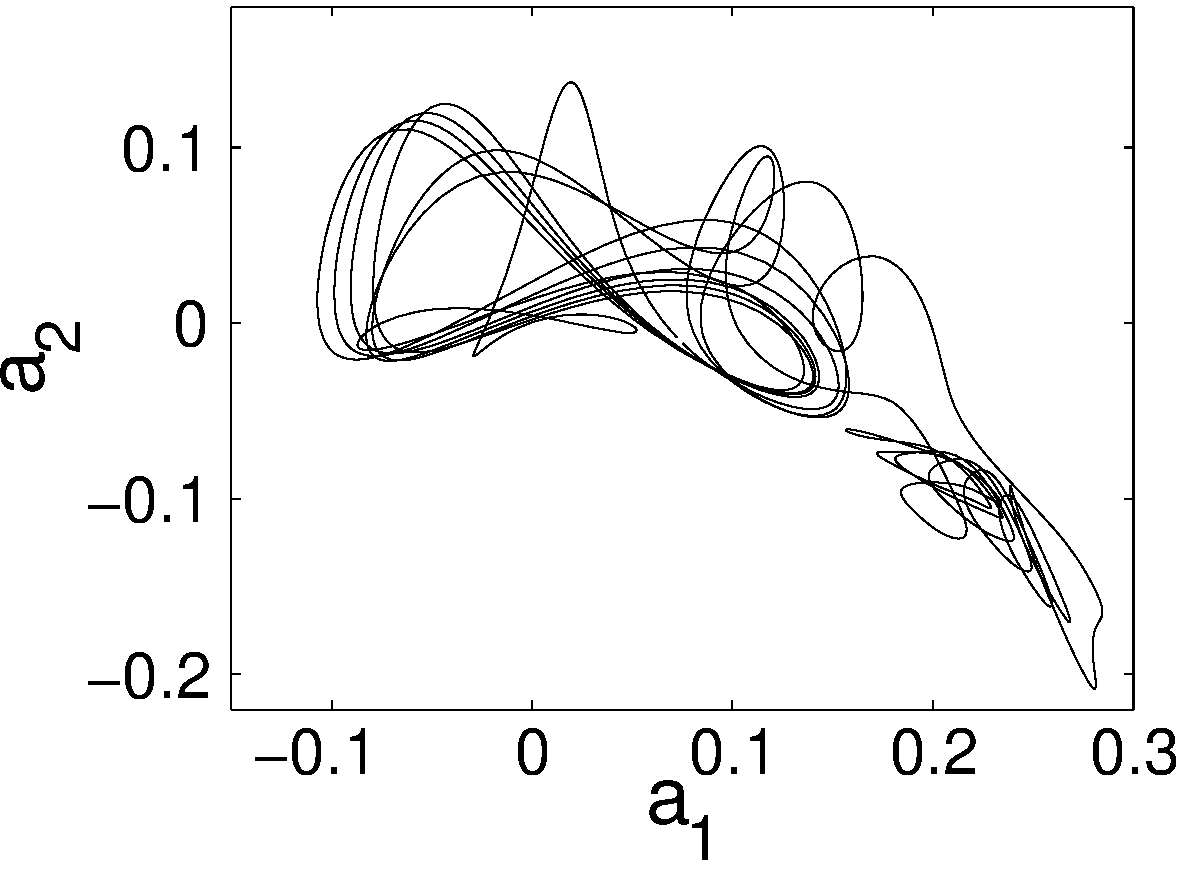
\includegraphics[width=0.40\textwidth]{kslong12}
\caption[]{
A long \KS\ \po\ of period $\period{}=355.34$ that connects
neighborhoods called `$S_C$' and `$S_R$',
(c) $[a_1,a_2]$  projection on the first two spatial Fourier modes
(from \refref{lanCvit07}).
      }
\label{f:antlong}
\end{figure}
%%%%%%%%%%%%%%%%%%%%%%%%%%%%%%%%%%%%%%%%%%%%%%%%%%%%%%%%%%%%%%


\section{Section}
\label{s:cut}


As an example consider the  [blah blah],

%%%%%%%%%%%%%%%%%%%%%%%%%%%%%%%%%%%%%%%%%%%%%%%%%%%%%%%%%%%%%%%%%%%%%
\begin{figure}
%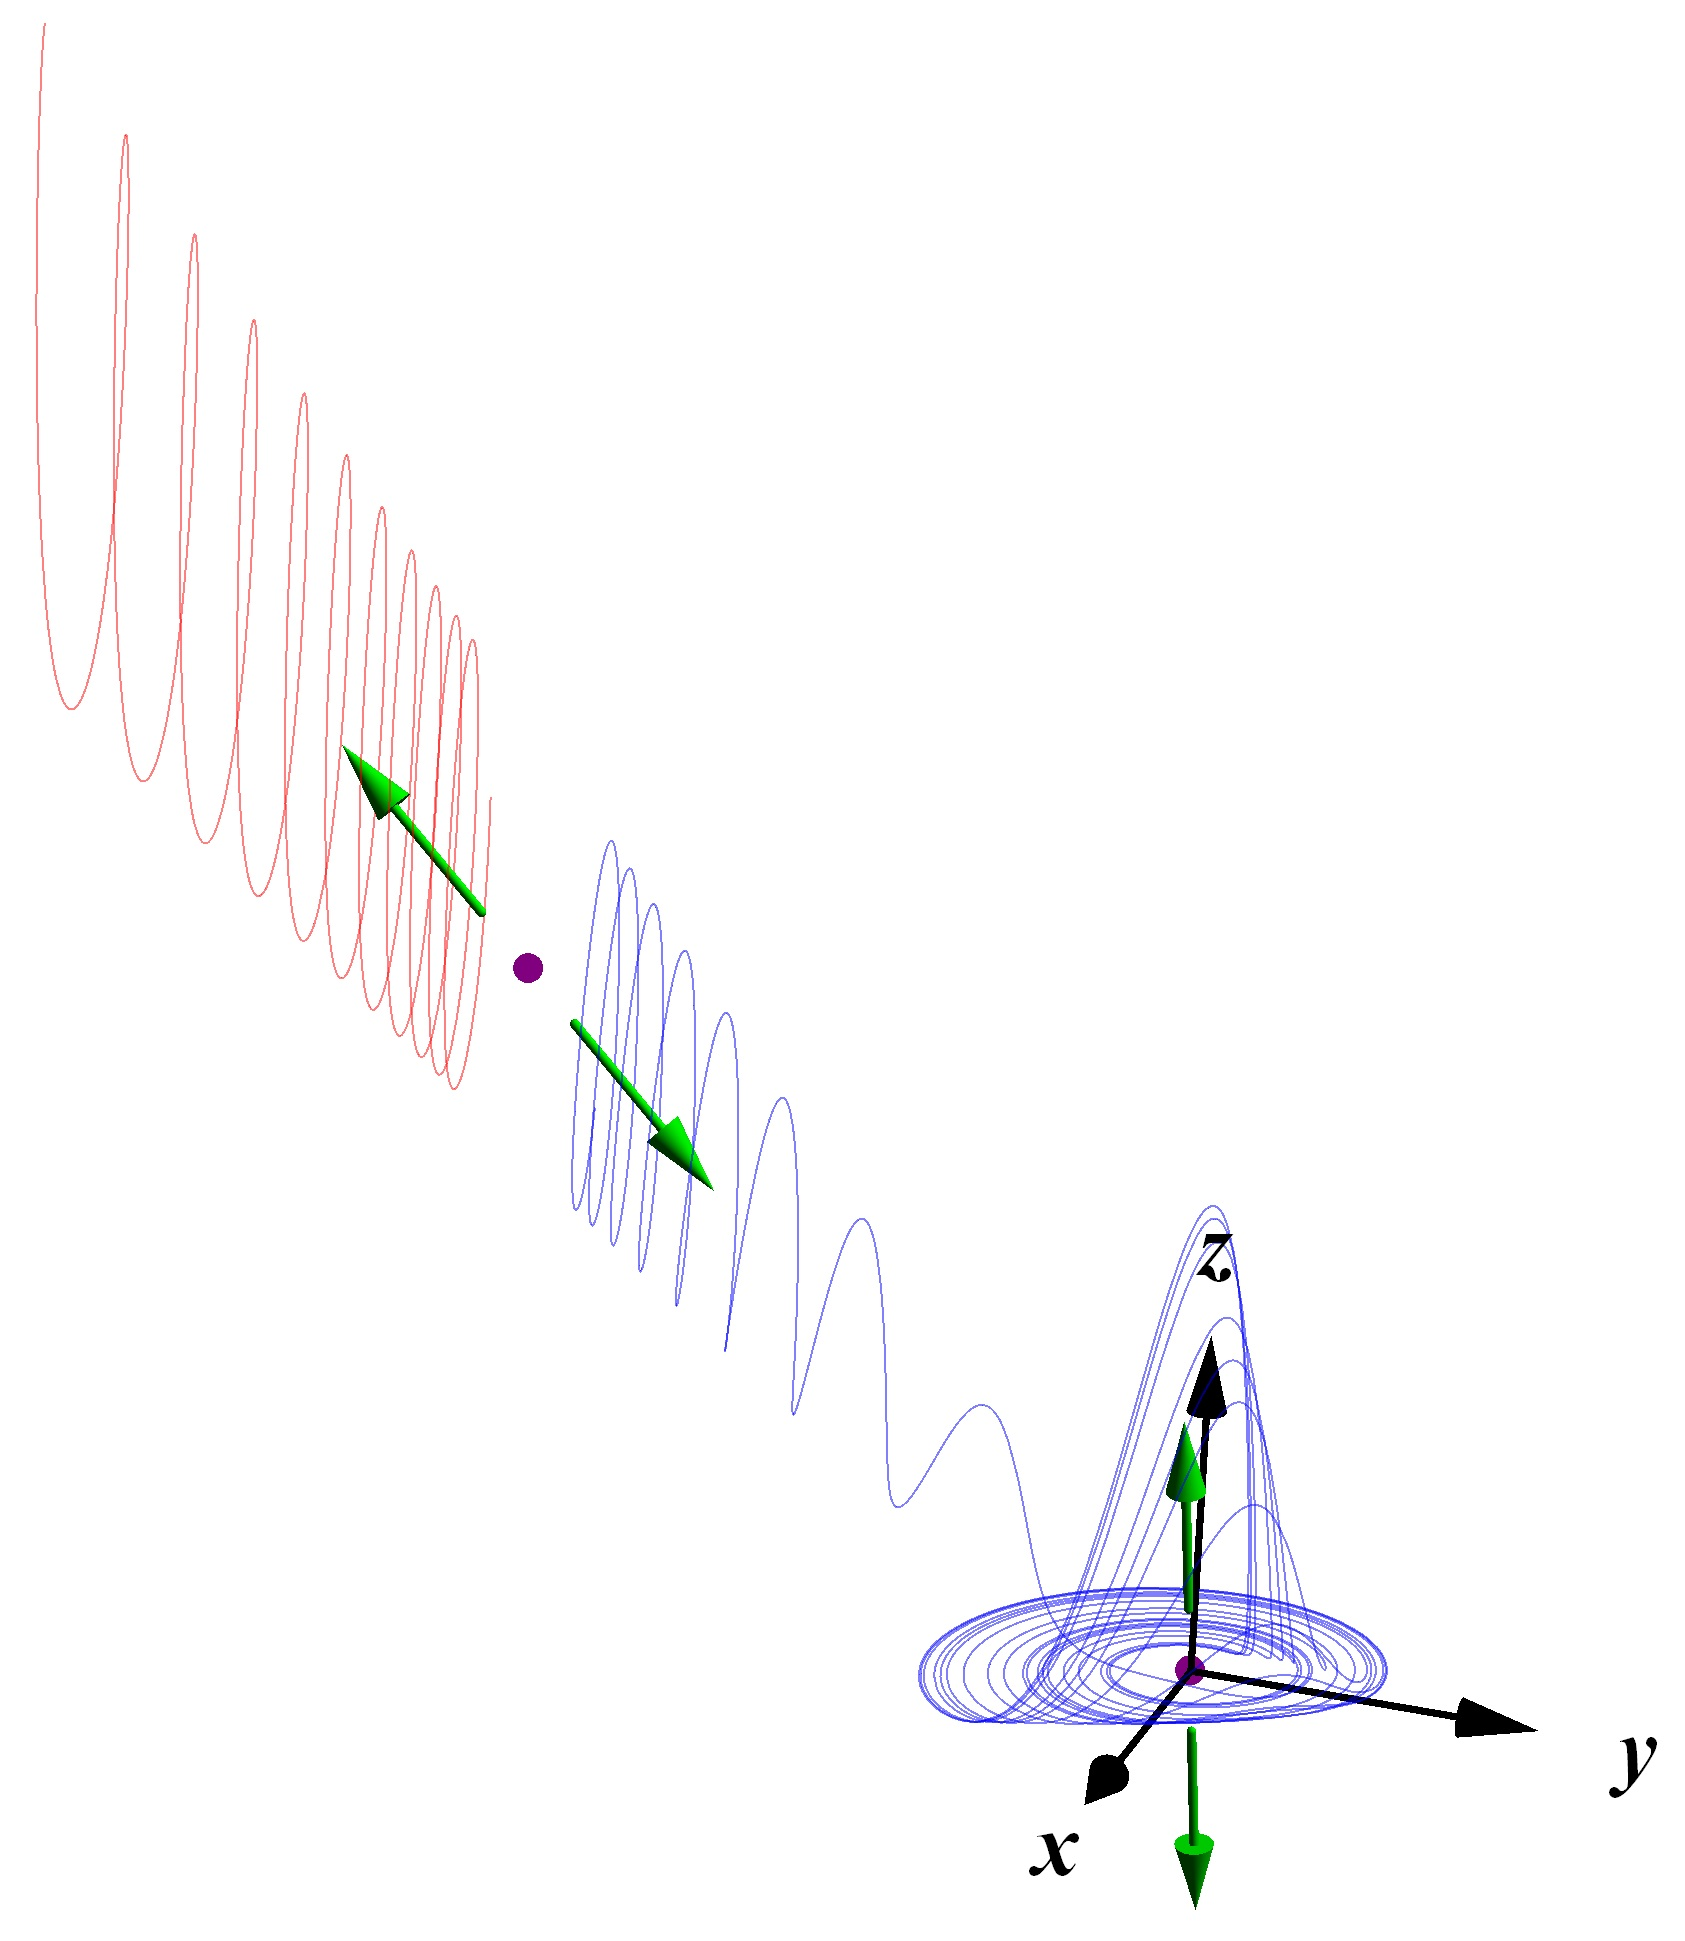
\includegraphics[width=0.28\textwidth]{RoessTrjs2}%{Rossler_Equilibria2}{RoessTrjs}%
 \begin{center}
 \setlength{\unitlength}{0.20\textwidth}
(a)
%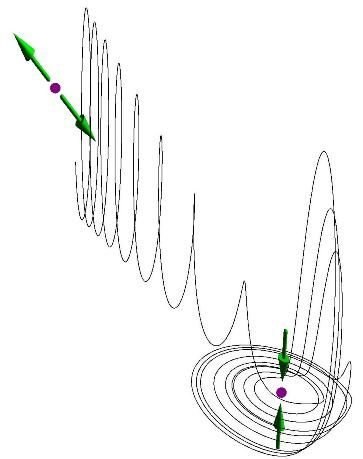
\includegraphics[width=\unitlength,clip=true]{RoessTrajLbld2}
(b)
%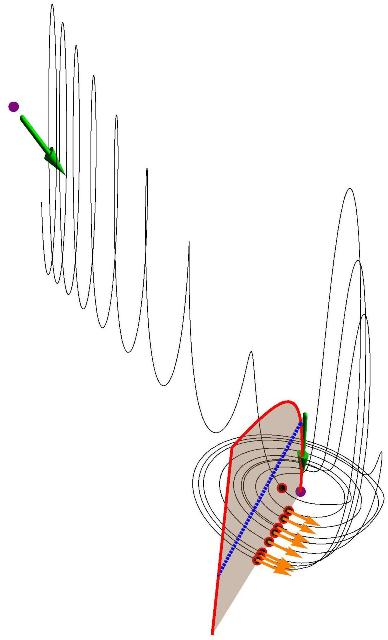
\includegraphics[width=\unitlength,clip=true]{RoessNeareqLbld2}
\\
(c)
%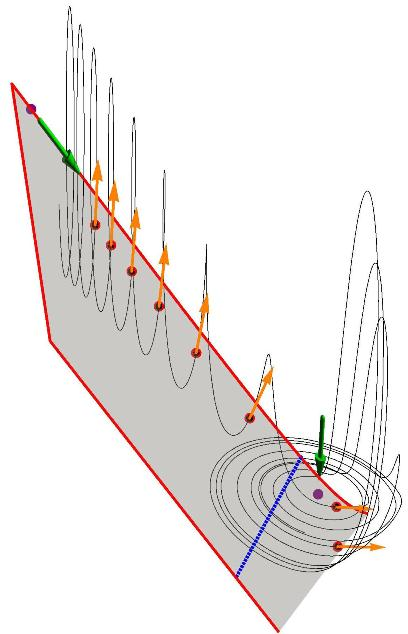
\includegraphics[width=\unitlength,clip=true]{RoessFareqLbld2}
(d)
%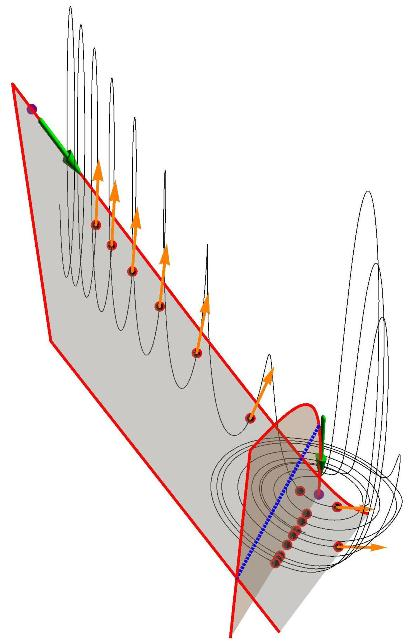
\includegraphics[width=\unitlength,clip=true]{RoessBotheqLbld2}
 \end{center}
    \caption{
2-chart atlas for \twoMode\ flow.
(a)
(b)
(c)
(d)
    }
\label{fig:2modeSects}
\end{figure}
%%%%%%%%%%%%%%%%%%%%%%%%%%%%%%%%%%%%%%%%%%%%%%%%%%%%%%%%%%%%%%%%%%%%%

 [blah blah]

\section{Dynamics and symmetry}
\label{s:symm}

\subsection{\twoMode\ $\SOn{2}$-equivariant flow}
\label{s:twoMode}

% \item[2012-04-28 Predrag]
Consider a system constructed from two Fourier modes
$m=(1,2)$,\rf{Dang86,AGHO288,PoKno05}, a representation of the symmetry
group $\SOn{2}$ defined by rotation
\beq
(z_1,z_2) \rightarrow   (e^{i {\gSpace}}z_1,e^{i 2{\gSpace}} z_2)
\,.
\ee{Dang86(1.1)aa}
$\SOn{2}$ invariant polynomials are
\bea
u &=& {z}_1 \overline{z}_1
    \,,\quad
v = {z}_2 \overline{z}_2
    \continue
w &=& z_1^2 \overline{z}_2 + \overline{z}_1^2 {z}_2
    \,,\quad
q = (z_1^2 \overline{z}_2 - \overline{z}_1^2 {z}_2)/\ii
\,,
\label{Dang86(1.2)PK}
\eea
The polynomials $\{u,v,w,q\}$ are
linearly independent, but related through one syzygy,
%2012-04-29 Double checked, added missing factors of 2 for w and q terms
%2012-04-29 Predrag: thanks!
\beq
w^2+q^2 - 4\,u^2v =0
  \,,
\label{eq:syzPK}
\eeq
confining the dynamics to a 3-dim\-ens\-ion\-al $\pS/\SOn{2}$ \reducedsp\
manifold, a
symmetry-invariant repre\-sent\-ati\-on of the 4-dim\-ens\-ion\-al
\SOn{2} equivariant dynamics.
The dynamical equations for $\{u,v,w,q\}$ follow from the chain rule
\( %beq
 \dot{ u}_i= ({\partial u_i}/{\partial x_j}) \, \dot{x}_j
 \,,
\) %ee{HilbChainRl}
upon substitution
$\{{z}_1\,,\overline{z}_1\,, {z}_2\,,\overline{z}_2 \}$ $\to$
$\{u,v,w,q\}$. This yields
\bea
  \dot{u} &=& \overline{z}_1 \dot{z}_1 + {z}_1 \dot{\overline{z}}_1 %Double checked DB 04-29-2012
\,,\qquad
  \dot{v} = \overline{z}_2 \dot{z}_2 + {z}_2 \dot{\overline{z}}_2 %Double checked DB 04-29-2012
\continue
  \dot{w} &=& 2 \,\overline{z}_2 {z}_1 \dot{z}_1 %Double checked DB 04-29-2012
           + 2\,{z}_2 \overline{z}_1 \dot{\overline{z}}_1
           + {z}_1^2 \dot{\overline{z}}_2
           + \overline{z}_1^2 \dot{z}_2
\continue
  \dot{q} &=&  (2\,\overline{z}_2 {z}_1 \dot{z}_1 %Double checked DB 04-29-2012
           - 2\,{z}_2 \overline{z}_1 \dot{\overline{z}}_1
           + {z}_1^2 \dot{\overline{z}}_2
           - \overline{z}_1^2 \dot{z}_2
           )/\ii
\label{PKinvEqs}
\eea

Dangelmayr,\rf{Dang86} Armbruster, Guckenheimer and Holmes,\rf{AGHO288}
Jones and Proctor,\rf{JoPro87} and Porter and Knobloch\rf{PoKno05} (see
Golubitsky \etal\rf{golubII}, Sect. XX.1) have investigated bifurcations
in 1:2 resonance ODE normal form models to third order in the amplitudes.
We shall study here a model of that type
that we shall refer to as the {\twoMode} system:
\begin{subequations}\label{eq:DangSO2}
\begin{align}
  \dot{z}_1 &= (\mu_1\ESedit{-\ii\, e_1})\,z_1+a_1\,z_1|z_1|^2
  +b_1\,z_1|z_2|^2+c_1\,\overline{z}_1\,z_2
\\
  \dot{z}_2 &= (\mu_2-\ii\, e_2)\,{z_2}+a_2\,z_2|z_1|^2+b_2\,z_2|z_2|^2+c_2\,z_1^2
\,,
\end{align}
\end{subequations}
with $z_1,\,z_2$  complex, and real valued  parameters. For parameters
far from bifurcation values the model has no physical motivation; in
particular, the parameter $(\mu_2-\ii\, e_2)$ is one of the many ways in
which $\On{2}$ symmetry of the Dangelmayr,\rf{Dang86} normal form system
can be broken to $\SOn{2}$ symmetry. We use the model to compare and
illustrate different symmetry reduction methods, in the dimensionally
lowest possible setting: a \statesp\ of dimension $d=4$, with the
$\SOn{2}$-reduced dynamics taking place in 3 dimensions, the lowest
possible if the dynamics is to be chaotic. Substituting the
$\SOn{2}$-equivariant system \refeq{eq:DangSO2} into \refeq{PKinvEqs} we
obtain a set of 4 invariant equations,
%    \PC{2012-04-27 to Lei and all, please recheck! $e_2$ terms differ
%    from Lei. DB 04-29: Double checked using computer algebra. Found a
%    couple of discrepancies. Fixed them in red.}
\bea% Triple checked ES 04-30-2012
  \dot{u} &=& 2\,\mu_1\,u+2\,a_1\,u^2+2\,b_1\,u\,v+c_1\,w %Double checked DB 04-29-2012
\continue
  \dot{v} &=& 2\,\mu_2\,v+2\,a_2\,u\,v+2\,b_2\,v^2+c_2\,w %Double checked DB 04-29-2012
\continue
  \dot{w} &=& (2\,\mu_1+\mu_2)\,w+(2a_1+a_2)\,u\,w+(2b_1+b_2)\,v\,w %Double checked DB 04-29-2012 corrected coefficients for uv and u^2 terms
\ceq
             +\, 4c_1\,u\,v + 2c_2\,u^2 +(\ESedit{2e_1} - e_2)\,q
\label{PKinvEqs1}\\
  \dot{q} &=& (2\mu_1+\mu_2)\,q+(2a_1+a_2)\,u\,q
\ceq
             +(2b_1+b_2)\,v\,q
             -(\ESedit{2e_1}-e_2)\,w %Double checked DB 04-29-2012
\,.
\nnu
\eea
The connection of the constants in \refeq{PKinvEqs1} %eq:2modesDangSO2}
with $e_2=0$ to the constants in
equation (2.3) of \refref{Dang86} with $n=2$, $m=1$ is $\mu_1=\nu\epsilon\alpha$,
$a_1=-\nu\epsilon$, $b_1=-\nu\epsilon\rho$, $c_1=-\nu\mu$, $\mu_2=\epsilon\beta$,
$a_2=-\epsilon\kappa$, $b_2=-\epsilon\epsilon'$, $c_2=\mu\mu'$.

One can now either investigate the dynamics in this invariant basis or
plot the `image'\rf{GL-Gil07b} of solutions computed in the equivariant
basis \refeq{eq:DangSO2} in terms of invariant polynomials
\refeq{Dang86(1.2)PK}.

%[2012-07-31 Evangelos]
Using the syzygy $w^2+q^2-4u^2v=0$ we can
eliminate $q$ from \refeq{PKinvEqs} to get
\bea% Triple checked ES 04-30-2012
  \dot{u} &=& 2\,\mu_1\,u+2\,a_1\,u^2+2\,b_1\,u\,v+c_1\,w %Double checked DB 04-29-2012
\continue
  \dot{v} &=& 2\,\mu_2\,v+2\,a_2\,u\,v+2\,b_2\,v^2+c_2\,w %Double checked DB 04-29-2012
\continue
  \dot{w} &=& (2\,\mu_1+\mu_2)\,w+(2a_1+a_2)\,u\,w+(2b_1+b_2)\,v\,w %Double checked DB 04-29-2012 corrected coefficients for uv and u^2 terms
\ceq
             +\, 4c_1\,u\,v + 2c_2\,u^2 +(2e_1 - e_2)(4u^2v-w^2)^{1/2}\,
\label{PKinvEqs1syz}
\eea
In polar coordinates $ {z}_1 = |u|^{1/2} e^{\ii\theta_1}$, $ {z}_2 =
|v|^{1/2} e^{\ii\theta_2}$ the  $w, q$ invariants take form
\bea
w &=& 2\,\Re(z_1^2 \overline{z}_2) = 2\,u |v|^{1/2} \cos \psi %Double checked DB 04-29-2012
\continue
q &=& 2\,\Im(z_1^2 \overline{z}_2) = 2\,u |v|^{1/2} \sin \psi %Double checked DB 04-29-2012
\,,
\label{Dang86(1.2)polar}
\eea
where $\psi = 2 \theta_1 - \theta_2$.


By substituting $z_1 = x_1 + i x_2$, $z_2 = y_1 + i y_2$, the complex
\twoMode\ system \refeq{eq:DangSO2} may be rewritten as a 4-dimensional
first order ODE system
\bea
\dot{x}_1 &=& \mu_1 x_1 + a_1 x_1^3 + b_1 x_1 y_1^2 + c_1 x_1 y_1 + a_1 x_1 x_2^2 + b_1 x_1 y_2^2
                              + c_1 x_2 y_2
\continue
\dot{x}_2 &=& \mu_1 x_2 + a_1 x_1^2 x_2 + c_1 x_1 y_2 + b_1 y_1^2 x_2 - c_1 y_1 x_2 + a_1 x_2^3
                         + b_1 x_2 y_2^2
\continue
\dot{y}_1 &=& \mu_2 y_1 + a_2 x_1^2 y_1 + c_2 x_1^2 + b_2 y_1^3 + a_2 y_1 x_2^2 + b_2 y_1 y_2^2
                        - c_2 x_2^2 + e_2 y_2
\continue
\dot{y}_2 &=& \mu_2 y_2 + a_2 x_1^2 y_2 + 2 c_2 x_1 x_2 + b_2 y_1^2 y_2 - e_2 y_1 + a_2 x_2^2 y_2
                        + b_2 y_2^3
\label{2mode4D}
\eea
%\item[2012-04-29 Predrag]
For the 4\dmn\ model at hand are using the invariant polynomials
$\{u,v,w,q\}$ dynamics only to develop intuition, but to illustrate the
general \mslices, everything has to do be done in $\pS =
\{x_1,x_2,y_1,y_2\}$ and \slice\ $\pSRed$ as well. You can see that even
for the simplest conceivable $\SOn{2}$ 4-dimensional flow one has to
think about how to construct the invariant polynomial basis, and it is
hard to imagine how anyone could do that for very high\dmn\ flows.

The {\stabmat} $\Mvar = {\pde \vel}/{\pde \ssp}$ for this 				
system is given by
% \PC{2012-06-11 reformat this}
\footnotesize
\begin{widetext}
\beq
\Mvar  \, =
\left( \begin{array}{cccc}
         (3 a_1 x_1^2 + b_1 y_1^2 + c_1 y_1 \\ + a_1 x_2^2 + b_1 y_2^2 + \mu_1) &  c_1 y_2 + 2 a_1 x_1 x_2 & c_1 x_1 + 2 b_1 x_1 y_1 & c_1 x_2 + 2 b_1 x_1 y_2 \\
        c_1 y_2 + 2 a_1 x_1 x_2  & a_1 x_1^2 + b_1 y_1^2 - c_1 y_1 + 3 a_1 x_2^2 + b_1 y_2^2 + \mu_1 & 2 b_1 y_1 x_2 - c_1 x_2 & c_1 x_1 + 2 b_1 x_2 y_2 \\
          2 c_2 x_1 + 2 a_2 x_1 y_1 & 2 a_2 y_1 x_2 - 2 c_2 x_2  & a_2 x_1^2 + 3 b_2 y_1^2 + a_2 x_2^2 + b_2 y_2^2 + \mu_2 & e_2 + 2 b_2 y_1 y_2\\
          2 c_2 x_2 + 2 a_2 x_1 y_2 & 2 c_2 x_1 + 2 a_2 x_2 y_2 & 2 b_2 y_1 y_2 - e_2 & (a_2 x_1^2 + b_2 y_1^2 + a_2 x_2^2 \\&&& + 3 b_2 y_2^2 + \mu_2)
      \end{array} \right)
\,.
\ee{2modeStabMatrix}
\end{widetext}
\normalsize
That the \twoMode\ system is equivariant under infinitesimal $\SOn{2}$
rotations is easily checked by substituting the Lie algebra generator
    \beq
\Lg  \, =
\left( \begin{array}{cccc}
         0 & 1 & 0 & 0 \\
        -1 & 0 & 0 & 0 \\
         0 & 0 & 0 & 2\\
         0 & 0 & -2 & 0
      \end{array} \right)
\ee{LGTwoMode}
and the {\stabmat} $\Mvar$ given in \refeq{2modeStabMatrix} into into the
equivariance condition
\beq
  \groupTan_a(\vel)  - \Mvar(\ssp) \, \groupTan_a(\ssp) =0
  \,.
\ee{inftmInv}
%
%%%%%%%%%%%%%%%%%%%%%%%%%%%%%%%%%%%%%%%%%%%%%%%%%%%%%%%%%%%
    \PC{this text copied from ChaosBook.org continuous.tex}
For a \reqv\ flow and group tangent vectors coincide,
$
\vel = \velRel \cdot \groupTan(\ssp)
\,.$
Dotting by the velocity $c$ (\ie, summing over $\velRel_a \groupTan_a$)
the equivariance condition \refeq{inftmInv},
$
\groupTan_a(\vel)  - \Mvar(\ssp) \, \groupTan_a(\ssp) =0
$,
we get
\beq
(\velRel \cdot \Lg - \Mvar ) \vel =0
\,.
\ee{ReqvMargEig}
In other words, in the co-rotating frame the eigenvalues corresponding to
group tangent are marginal, and the velocity $\vel$ is the corresponding
right eigenvector.
%%%% up to here text copied from ChaosBook.org continuous.tex

\subsection{\Eqva}
\label{s:eqva}

%[2012-04-28 Predrag]
How to solve for \eqva\ of \refeq{PKinvEqs}? Define
\beq
A_1= \mu_1+a_1\,u+b_1\,v
    \,,\qquad
A_2 = \mu_2+a_2\,u+b_2\,v
\ee{PKinvEqs2a}
then rewrite \refeq{PKinvEqs} as
%     \newpage
\bea
  0  &=&  2\,A_1\,u +c_1\,w
    \,,\qquad
  0  =  2\,A_2\,v +c_2\,w
\continue
  0  &=& (2\,A_1+ A_2)\,w
             +2\,\left(c_2\,u+2\,c_1\,v\right)\,u -e_2\,q
\label{PKinvEqs3}\\
  0  &=& (2\,A_1+ A_2)\,q + e_2\,\,w
\nnu
\eea
We already know $[0,0,0,0]$ and $[0,v,0,0]$ roots, so we are looking only
for the $u>0$, $v>0$, $w,q \in \reals$ solutions; there could be problems
from the non-generic roots with either $w=0$ or $q=0$, but not both
simultaneously, syzygy \refeq{eq:syzPK} precludes that. $w$ and/or $q$
can be eliminated by rewriting \refeq{PKinvEqs3} as:
\bea
  w  &=& - \frac{2\,u}{c_1}\,A_1 = - \frac{2\,v}{c_2}\,A_2
\continue
        &\to&\quad 2\,A_1+ A_2 = - \frac{ w}{2\,u\,v}\left(c_2\,u+2\,c_1\,v\right)
\continue
  q  &=& \frac{1}{\ESedit{-2e_1+}e_2}
     \left(- {w^2}/{2\,u\,v} + \,2u\right)\left(c_2\,u+2\,c_1\,v\right)
\label{PKinvEqs4}\\
  w  &=& -\frac{1}{\ESedit{-2e_1+}e_2} (2\,A_1+ A_2)\,q
     \,,\quad\to\quad
  q = \frac{2(\ESedit{-2e_1+}\,e_2)\,u\,v}{c_2\,u+2\,c_1\,v}
  \,,
\nnu
\eea
%\DBedit{DB: Not sure where this factor of 2 comes from in $w =
%-\frac{2}{e_2} (2\,A_1+ A_2)\,q $. From the last equation in
%\refeq{PKinvEqs3}, I get $w = -\frac{1}{e_2} (2\,A_1+ A_2)\,q$.
%Therefore, I get I get  $q = \frac{2 e_2\,u\,v}{c_2\,u+2\,c_1\,v}$}
%2012-04-29 Predrag: thanks!
and thus we obtain \textbf{our main result}, two (bivariate)  polynomials
in two variables $\{u,v\}$ with constant coefficients
\bea
f(u,v) &=&
  c_2\,u\,(\mu_1+a_1\,u+b_1\,v)
     -
  c_1\,v\,(\mu_2+a_2\,u+b_2\,v) = 0 %Double checked DB 04-30-2012
\,,\qquad  deg(f) = 2
\continue
g(u,v) &=&
 \left(w^2 - 4\,u^2 v\right)\left(c_2\,u+2\,c_1\,v\right)^2 %Double checked DB 04-30-2012
 +\,4\,(\ESedit{-2e_1+}e_2)^2\,u^2\,v^2 = 0
\,,\qquad  deg(g) = 6
\,,
\label{PKinvEqs5}
\eea
% \DBedit{DB: I get $g(u,v) = \left(w^2 - 4\,u^2
% v\right)\left(c_2\,u+2\,c_1\,v\right)^2 +\,4\,e_2^2\,u^2\,v^2 = 0$}
%2012-04-29 Predrag: thanks!
%2012-04-29 Predrag: should have I used the syzygy \refeq{eq:syzPK},
%$w^2 - 4\,u^2v = -q^2$ DB: If you plug the syzygy in you trivially get zero....
where if $w$ should be substituted as defined by the first equation in
\refeq{PKinvEqs4}.
Lots of coefficients, but we can
absorb some into rescaled quantities
$\tilde{u} = c_2\,u$,
$\tilde{v} = c_1\,v$,
$\tilde{a_1} = a_1/c_2$,
$\tilde{b_1} = b_1/c_1$,
$\tilde{a_2} = a_2/c_2$,
$\tilde{b_2} = b_2/c_1$,
and by using $A_1$ expression for $w$ factored out the pair of $u=0$
roots:
\bea
\tilde{f}(\tilde{u},\tilde{v}) &=&
  \tilde{u}\,A_1 - \tilde{v}\,A_2 = 0 %Double checked DB 04-30-2012
\,,\qquad\qquad\qquad  deg(f) = 2
\continue
\tilde{g}(\tilde{u},\tilde{v}) &=&  %Double checked DB 04-30-2012
 \left(A_1^2
 - c_1\,\tilde{v}\right)
 \left(\tilde{u}+2\,\tilde{v}\right)^2
 +e_2^2\,\tilde{v}^2 = 0
\,,\qquad  deg(g) = 4
\continue
 && \mbox{where }
A_1 = \mu_1+\tilde{a_1}\,\tilde{u}+\tilde{b_1}\,\tilde{v}
\,,\quad
A_2 = \mu_2+\tilde{a_2}\,\tilde{u}+\tilde{b_2}\,\tilde{v}
\,,
\label{PKinvEqs5a}
\eea
so we are down to 8 coefficients. Note that $e_2 \in \reals_{+}$, and if
we agree that  $\mu_1 > -\mu_2 > 0$ vi can rescale the first equation so
that in new time units $\tilde{\mu}_1 =1$, $\tilde{\mu}_2 = \mu_2/\mu_1
\in \reals_{-}$, so there are 7 coefficients in all. I see no further
rescaling simplification.

As we already know $[0,0,0,0]$ and $[0,v,0,0]$ roots, one should divide
them out, and that is what we have done. Finding
roots of bivariate polynomials is not easy.

At the origin $\Mvar$ commutes with $\Lg$, and thus can be block-diagonalized
into two $[2\!\times\!2]$ matrices.
% According to {\bf [2012-04-27 Daniel]},
The $[0,0,0,0]$ \eqv\ eigenvalues are $\lambda_1 = \mu_1$ with multiplicity 2 and
             $\lambda_3 = \mu_2 \pm i e_2$. The eigenvectors for
             $\lambda_1$ are $(1,0,0,0)$ and $(0,1,0,0)$ in the
             $(x_1,x_2,y_1,y_2)$ basis.
             The eigenvectors for
             $\lambda_2$ are $(0,0,1,0)$ and $(0,0,0,1)$


%%%%%%%%%%%%%%%%%%%%%%%%%%%%%%%%%%%%%%%%%%%%%%%%%%%%%%%%%%%%%%%%%%%%%%%%%%%%%%%%%%%%%%%%%%%%%%%%%%
\subsection{To do}
\label{s:ToDo}

\begin{itemize}
  \item[10.11] Visualizations of the 4-dimensional {\twoMode} system
  \item[10.1?] draw a group orbit for the {\twoMode} model
  \item[10.22] {\twoMode} system in polar coordinates (maybe skip)
  \item[10.23] The \reqva\ of the {\twoMode} system
  \item[10.24] Plotting the \reqva\ of
           the {\twoMode} system in invariant coordinates
  \item[10.25] Plotting the \reqva\ of
           the {\twoMode} system in Cartesian coordinates
           \refeq{2mode4D}
  \item[10.2?] construct a 2-chart atlas
           \reffig{fig:2ModeAtlas} for a {\twoMode} system
  \item
        compute analytically the \stabmat\ \Mvar\ in polar coordinates
  \item
        Study eigenvalues, keep playing with parameters. We would like
        -preferably- no \reqv\ to be attracting limit cycle, and several of
        the \reqva\ to be complex-pair unstable, leading to chaos, to be
        visualized and sliced in Cartesian coordinates.
  \item
        If you find a nice chaotic attractors, others can join in
        constructing an atlas for it. We just need one and only one
        example with non-trivial \chartBord s and at least 2 charts.
\end{itemize}

 [blah blah]

\begin{itemize}
  \item $\REQV{}{1} = (r_1,r_2,\psi)=(0.0516508, 1.26311,?)$ and
        $\REQV{}{2} = (0.467095,0.2146,?)$
  \item their plots in the Cartesian coordinates
  \item $\dot{\theta}$ to see how slow/fast are they. $\dot{\theta}$
        might be related to 4th eigenvalue, when you go back
        to Cartesian coordinates
  \item stability eigenvalues, eigenvectors of the \eqv\ $\EQV{0}$ at
        origin, at your parameter values - if it is stable, everything
        just might fall into it and die.
  \item plots of small perturbations of the above \eqv\ and \reqva\ in
        the Cartesian coordinates to see whether the dynamics looks
        chaotic
  \item $\REQV{}{1}$: 2 large positive eigenvalues looks scary - probably
        nothing re-visits this \reqv. A mildly unstable complex pair
        would have been sweeter. You get complex eigenvalue by Hopf-bifurcating off a
        stable orbit, typically.
  \item $\REQV{}{1}$: Does either unstable eigenvalue become a complex
        eigenvalue pair in Cartesian coordinates?
  \item $\REQV{}{2}$: contracting eigenvalues have very small imaginary
        part, so the presumably just rocket toward the \reqv, not much
        spiraling there. At least the unstable eigenvalue seems slow
        compared to all other eigenvalues.
  \item $\REQV{}{1}$: Does the unstable eigenvalue become a complex
        eigenvalue pair in Cartesian coordinates?
\end{itemize}

 [blah blah]



%%%%%%%%%%%%%%%%%%%%%%%%%%%%%%%%%%%%%%%%%%%%%%%%%
% 2011-09-09, 2012-03-30 Predrag: add BeThMovFr to
%            continuous.tex overheads, and ChaosBook
% replace A27movFrame*.* everywhere
\begin{figure}
  	\begin{center}
  	\setlength{\unitlength}{0.20\textwidth}
  (a)
  	\begin{picture}(1,1.07802818)%
    	\put(0,0){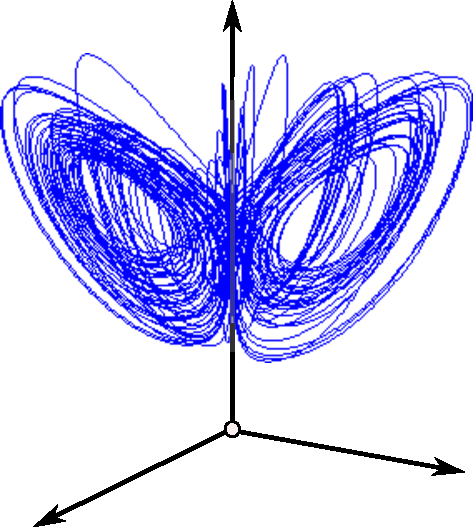
\includegraphics[width=\unitlength]{CLEattractor}}%
    	\put(0.55152995,1.0139628){\color[rgb]{0,0,0}\makebox(0,0)[lb]{\smash{$z$}}}%
    	\put(0.05573445,0.0739776){\color[rgb]{0,0,0}\makebox(0,0)[lb]{\smash{$x_1$}}}%
    	\put(0.90013492,0.16491708){\color[rgb]{0,0,0}\makebox(0,0)[lb]{\smash{$x_2$}}}%
  	\end{picture}%	
  (b)
  	\begin{picture}(1,1.06440474)%
    	\put(0,0){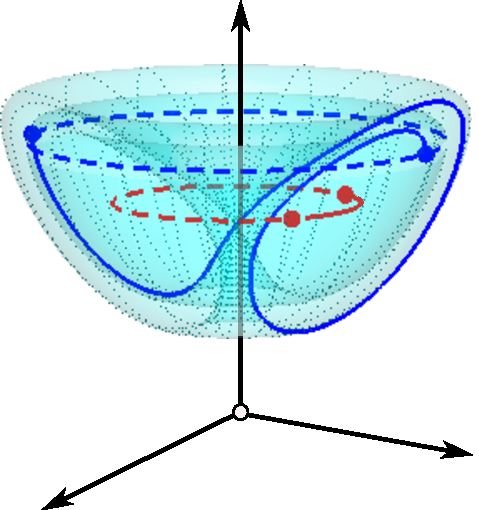
\includegraphics[width=\unitlength]{CLEWurst01}}%
   		\put(0.55961552,1.00214901){\color[rgb]{0,0,0}\makebox(0,0)[lb]{\smash{$z$}}}%
   		\put(0.07008555,0.07304272){\color[rgb]{0,0,0}\makebox(0,0)[lb]{\smash{$x_1$}}}%
    	\put(0.90381504,0.16283301){\color[rgb]{0,0,0}\makebox(0,0)[lb]{\smash{$x_2$}}}%
  	\end{picture}
\\
(c)   \begin{picture}(1,0.94310243)%
    \put(0,0){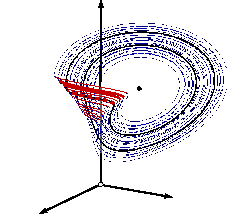
\includegraphics[width=\unitlength]{CLE1SliceSmall}}%
    \put(0.48564392,0.89244183){\color[rgb]{0,0,0}\makebox(0,0)[lb]{\smash{$z$}}}%
    \put(0.07181137,0.03185892){\color[rgb]{0,0,0}\makebox(0,0)[lb]{\smash{$y_2$}}}%
    \put(0.77031544,0.100183){\color[rgb]{0,0,0}\makebox(0,0)[lb]{\smash{$x_2$}}}%
  \end{picture}%
(d)   \begin{picture}(1,1.05662086)%
    \put(0,0){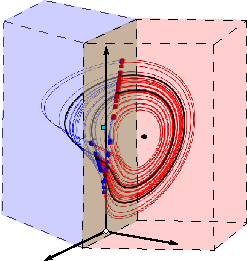
\includegraphics[width=\unitlength]{CLE2slicesmall}}%
    \put(0.47706962,0.83002768){\color[rgb]{0,0,0}\makebox(0,0)[lb]{\smash{$z$}}}%
    \put(0.08719004,0.02997825){\color[rgb]{0,0,0}\makebox(0,0)[lb]{\smash{$y_2$}}}%
    \put(0.73025395,0.09287946){\color[rgb]{0,0,0}\makebox(0,0)[lb]{\smash{$x_2$}}}%
  \end{picture}
    \end{center}
  \caption{
  \twoMode, $d=4 \to 3$~dimensional $\{x_1,x_2,z\}$ projections:
  (a)
  The strange attractor.
  (b)
 (c)
 In contrast
 to the 1\dmn\ \poincBord s of \reffig{fig:2modeSects}, here ...
 (d)
  }
\label{fig:2ModeAtlas}
\end{figure}
%%%%%%%%%%%%%%%%%%%%%%%%%%%%%%%%%%%%%%%%%%%%%%%%%%

 [blah blah]

 [blah blah]

\section{Chart}
\label{s:slice}

 [blah blah]

One can write the equations for the flow in the \reducedsp\
$\dot{\sspRed} = \velRed(\sspRed)$ (for details see, for example,
\refref{DasBuch}) as
\bea
\velRed(\sspRed) &=& \vel(\sspRed)
     \,-\, \dot{\gSpace}(\sspRed) \, \groupTan(\sspRed)
\label{2modesEqMotMFrame}\\
\dot{\gSpace}(\sspRed) &=& \braket{\vel(\sspRed)}{\sliceTan{}}
                       /\braket{\groupTan(\sspRed)}{\sliceTan{}}
\,
\label{2modesreconstrEq}
\eea
which confines the motion to the \slice\ hyperplane. Thus, the dynamical
system $\{\pS,\map^t\}$ with continuous symmetry \Group\ is replaced by
the {\reducedsp} dynamics $\{\pSRed,\mapRed^t\}$: The velocity in the
full \statesp\ $\vel$ is the sum of $\velRed$, the velocity component in
the \slice\ hyperplane, and $\dot{\gSpace}\,\groupTan$, the velocity
component along the group tangent space. The integral of the {\em
reconstruction equation} for $\dot{\gSpace}$ keeps track of the group
shift in the full \statesp.


 [blah blah]

\section{Charting the \slice}
\label{s:chart}

Let us summarize the voyage so far:

 [blah blah]


How the charts are put together is best told as a graphic tale, in the 5
frames of Figs.  [blah blah]



\section{Conclusions}
\label{s:concl}

 [blah blah]

\begin{acknowledgments}
This report addresses the questions asked in the  2012 Chaos course
[blah blah].
We are indebted to
Lei Zhang, Bryce Robbins,
and
Sarah Flynn
for many inspiring discussions and cross-checks of the model,
and Edgar Knobloch for [...].
\end{acknowledgments}


\bibliography{../bibtex/siminos}
%   \fi % 2012-08-06 end of temporary \onecolumngrid


\ifdraft
    \onecolumngrid

    \newpage
\input flotsam
    \newpage
    \section{{\twoMode} simulations blog}
    \label{chap:Mathematica}
\input ../blog/Mathematica

    \newpage
    \section{{\twoMode} daily blog}
    \label{chap:2modes}
\input ../blog/2modes
    \newpage
    \section{Burak' s {\twoMode}}
    \label{chap:2modes}
\input ../blog/2modesBB % Predrag 2013-0810 Burak, git version only

\addcontentsline{toc}{section}{last blog entry}

%\vfill
%\begin{quote}
%{\color{red} \large
%May 1 2012,  11:30am - 2:20pm term projects due, Predrag's office
%}
%\end{quote}

\fi

\end{document}
